\section{Architecture}\label{sec:architecture}


%In addition, we propose an initial reference implementation by selecting one or more solutions for each reference component. In particular, embracing the lean development approach, we detail only the core of the platform, namely the tools on which a strong convergence exists among the consortium members (the minimum viable product or MVP). The rest of the platform is constituted by suggestion of tools and/or technologies that at this moment seem to be good candidates but that may be replaced as the project develops. 


%The most significant requirement to be satisfied is adaptability, i.e. the architecture that we are about to describe must be able to apply without changes to all the planned pilots. This is indeed challenging as pilots are characterized by use scenarios, workflow and resources that may vary from one another; nevertheless, they all plan to exploit the data sets provided by the project partners (hereinafter referred to as Core Data) and specific solutions for data transformation, analytics and reporting.
For this reason, the various components of the reference architecture have been grouped into three macro areas:

\begin{itemize}
    \item Core Data Services: These components provide access to data made accessible by partners or freely available. These data sets are used in both data linking and enrichment processes.
    \item Platform Services: data preparation, analytics and visualization services. They are located at the top of the reference stack for Big Data architectures. The focus of the project is on these services, their integration and exploitation.
    \item Corporate Services: These components refer to tools for data ingestion, storage and processing, data flow and security management. In general, these components are found at the lowest levels of Big Data architectures and, moreover, in our case they depend heavily on the technologies present at customers' premises.  
\end{itemize}

As mentioned above, the first two groups are the central focus of the project. 
As far as the Corporate Services group is concerned, we will limit ourselves to indicating the main components and describing their functionalities in order to provide the reader with a comprehensive overview.  
The EW-Shopp ecosystem includes three macro components that relate to the preparation, analytics and visualization processes. 
EW-Shopp Corporate, on the other hand, presents the components needed to store large volumes of data, process them in a distributed and scalable way, data ingestion systems, data flow orchestration, and security, i.e. authentication, authorization, encryption and anonymization. 
 
\begin{figure}[t]
\centering
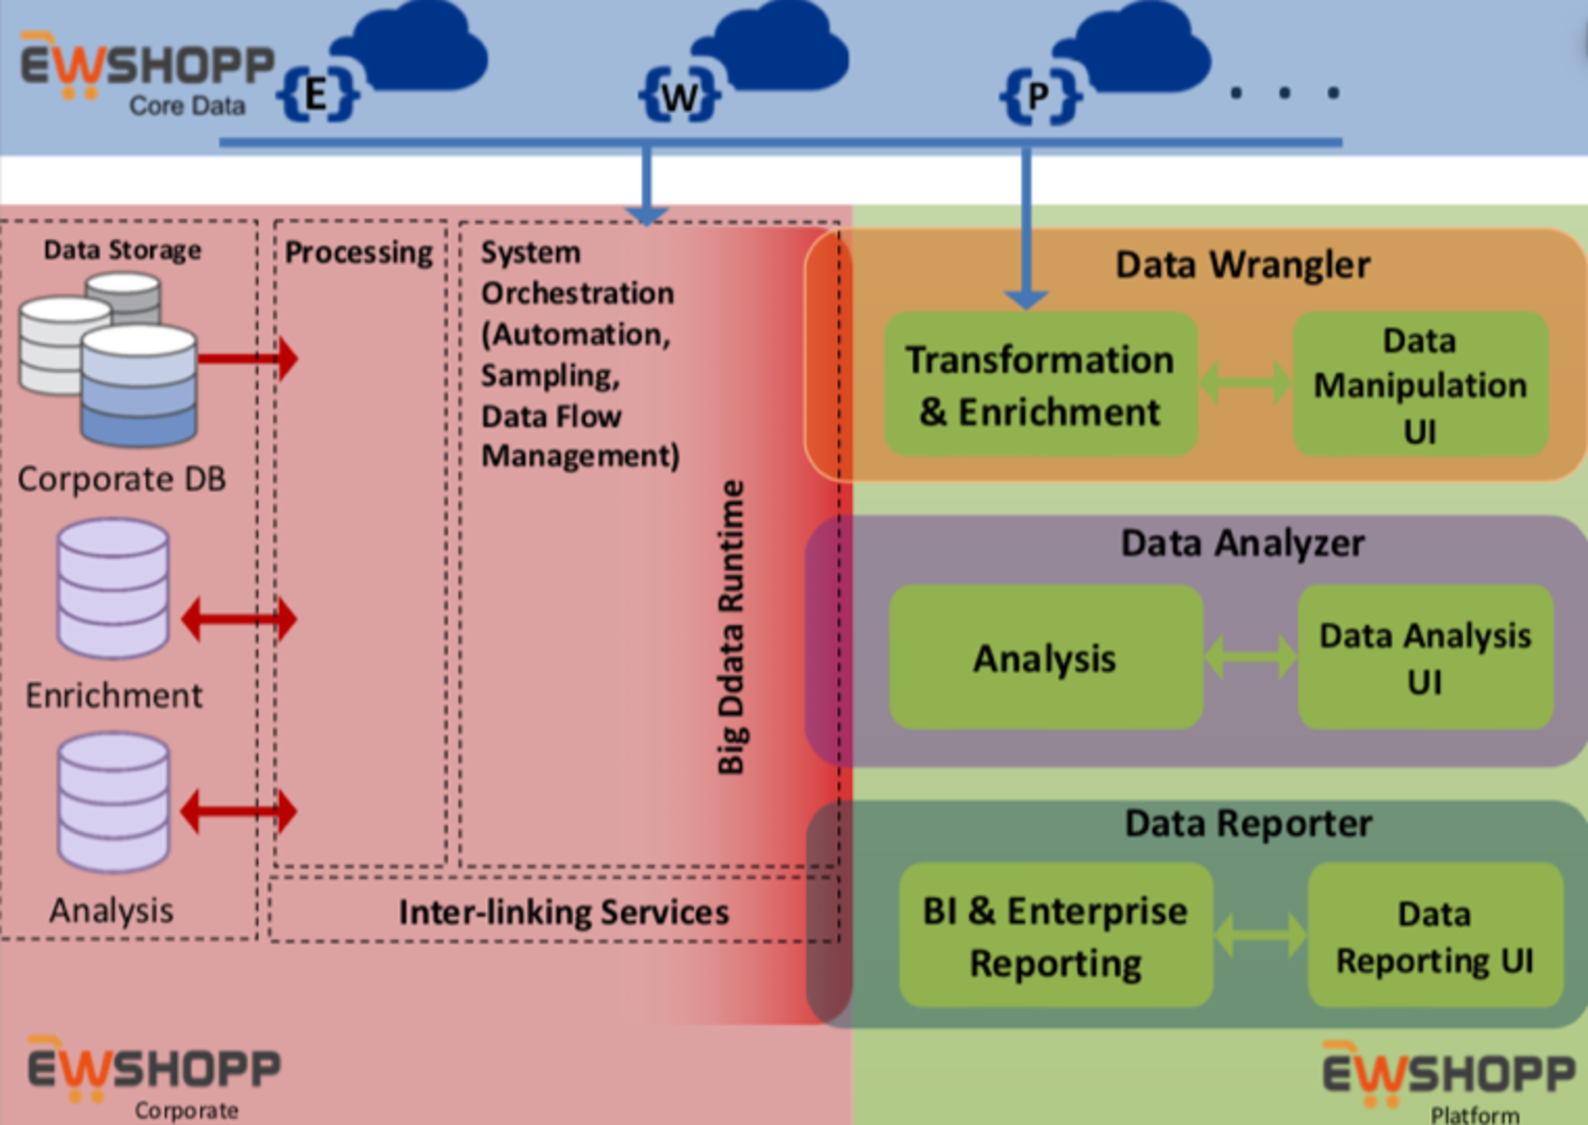
\includegraphics[width=\columnwidth]{figs/Architecture.pdf}
\vspace{-.3cm}
\caption{General architecture}
\label{fig:architecture} 
\end{figure}  

 
 
On the other hand, the focus in Figure 5 is exclusively on the components contributing to the EW-Shopp reference architecture. Unlike the solutions proposed by NIST or BDVA, the architecture that we describe in this document intentionally exclude the infrastructure layer, data ingestion and access layer. While these components will be considered in the implementation phase we believe that presenting and discussing them here would have added no value to the architecture specification, which aims to be especially focused on the large-scale execution of data preparation, analytics, and reporting tools belonging to the application layer (i.e. the NIST Big Data Application Provider).
Using the same color scheme used in Figure 4 as an interpretation guide, we specified the platform components at application level in Figure 5 . They are:
\begin{itemize}
    \item Data Wrangler (DW), which is the component that is designed to enable the user to define at design time the transformations of data cleaning, linking and enrichment. Such data preparation processes will then be carried out by the component referred to as Big Data Runtime.
    \item Data Analyzer (DA), which is the component that provides a set of predefined tools for predictive and prescriptive algorithms on enriched data. 
    \item Data Reporter (DR), which is the component that allows the user to visualize and analyze from a business point of view the outcomes produced by the Analyzer data.  
\end{itemize}
More details on this component and its implementation can be found in Section 4.2.3 and Section 5.4. As regards the so-called Corporate services, these are gathered in a single macro-component called Big Data Runtime (BDR). This part of the architecture provides the capability to execute transformation operations defined by the Data Wrangler and analytics operations of the Data Analyzer on large amounts of data. In addition, this component provides the data reporter with specific APIs for data access. Within the Big Data Runtime, we recognize (using the terminology proposed by NIST) a sub-component in charge of Data Storage and another dedicated to the Processing of such data. Moreover, we included in the picture a component responsible for orchestrating the processes to be performed and the data flow (System Orchestration). 
The architecture foresees the presence of crosscutting services to enforce appropriate security and monitoring policies (Security Services).
Unlike the previous picture, Figure 5 includes an area (in light blue) that groups together the components for the management of the Core Data. These are accessible via generic REST APIs. With no ambition for completeness, the figure shows the APIs for events, weather and products data. Other enrichment sources may include free data sets such as DBpedia .
Clearly, since the image in question does not constitute a deployment diagram, having presented the three logical sections of the architecture separately does not imply that they will be deployed independently and/or geographically apart. On the contrary, as we will see later on. The architecture, the control flow, and the dataflow pipeline have been conceived in such a way as to realize different typologies of deployments, from the completely distributed one in which the three logical regions are also physically separated and distant, to the centralized one in which the entire architecture is implemented within the same facility.
   




\subsection{Data Wrangler}
descrizione di come funziona.
messaggio, non un tool per esperti tecnologi ma esperti di dominio si.

Data to be imported will typically be in tabular format with varying quality with respect to missing values, invalid values, duplicated records, etc. Improving quality through data cleaning is important when different datasets are connected in the final data graph. When data quality is sufficient, the data can be transformed by selecting the important columns and rows through a filtering process. This can reduce the amount of data and make the dataset easier to store and query. The dataset will further be enriched with data from other domains like event/weather data. Depending on the application area, the dataset can be converted/mapped into graph of data. The mapping must be done according to an ontology and vocabulary for the data set. The mapping/annotation step is typically the most time consuming. The data is stored in an appropriate format for the receiving applications. A sample dataset is used for specifying and assessing the transformation and mapping steps using online tools. A transformation model is generated for batch execution on Big Data Runtime against the full dataset. 
Figure 7 shows a component diagram of the Data Wrangler tool with component interactions in terms of data exchanging. The image represents the most general case, i.e. where the data to be transformed is very large and managed by the corporate area of EW-Shopp. In this scenario, we apply the Dimension Reduction Approach presented in Section 4.2.1. The components of every logical area of the platform are involved. We have on the left the Data Wrangler Sampler, the summarizer and the engine that are components that interact with the Big Data Runtime to generate the sample to be used to define the transformations, to realize a set of suggestions for the table annotation process based on summarizations of existing knowledge bases or previous annotations, and finally to perform on a large scale the transformations defined by the user, respectively. The transformation process is defined by the user through a graphical interface that interacts with a backend service.
Both for the definition of the entire process (which requires the transformation of the work dataset) and for its actual execution on the business dataset, the Data Wrangler process may need data for disambiguation, linking and enrichment. These data are provided by the Core Data services.
 
Figure 7: Data Wrangler architecture




\subsection{Dataspace and Big Data Back end}
